\subsection{ADD/SUB}
\begin{frame}
    \frametitle{Addition/Subtraction}
    A selector can be designed so that either addition (ADD) or subtraction (SUB)
    can be performed using the same hardware when working with two's complement representations.
    Let's define the operands $x$ and $y$ with the following notations:
    \begin{equation}
        \begin{aligned}
            &\text{result} =
            \begin{cases}
                x + y, & \text{if ADD} \\
                x + (-y), & \text{if SUB}
            \end{cases}
        \end{aligned}
    \end{equation}
\end{frame}

% \begin{frame}
%     \frametitle{Addition/Subtraction}
% \end{frame}

\begin{frame}
    \frametitle{Adder}
    The various types of adder implementations in hardware include:
    \begin{itemize}
        \item Ripple Carry Adder
        \item Carry Lookahead Adder
            \begin{itemize}
                \item Carry Skip Adder (bypass)
                \item Carry Select Adder (multiplexer)
            \end{itemize}
    \end{itemize}
\end{frame}

\begin{frame}
    \frametitle{Half adder}
 A half adder is a combinational circuit that adds two bits and produces a sum and carry bits.
    \begin{figure}
        \centering
        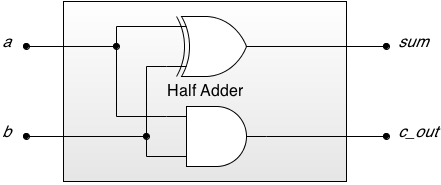
\includegraphics[width=0.7\textwidth]{media/half-adder-gates.png}
        \caption{Half Adder}
    \end{figure}
\end{frame}

\begin{frame}
    \frametitle{Full adder}
 A full adder is a combinational circuit that adds three bits and produces a sum and carry bits.
    \begin{figure}
        \centering
        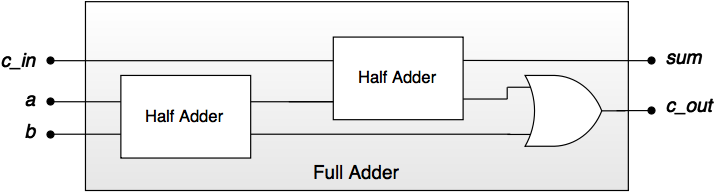
\includegraphics[width=0.7\textwidth]{media/full-adder-gates.png}
        \caption{Full Adder}
    \end{figure}
\end{frame}

\begin{frame}
    \frametitle{Ripple Carry Adder}
 The simplest adder is the ripple carry adder.
 It is composed of a chain of full adders.
 The carry-out of one full adder is the carry-in of the next full adder.
    \begin{figure}
        \centering
        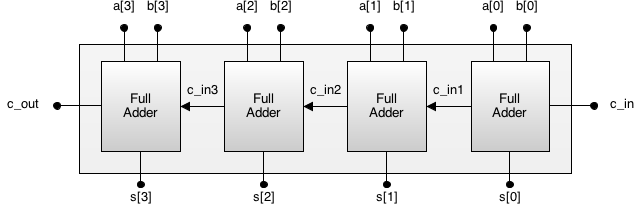
\includegraphics[width=0.7\textwidth]{media/ripple-carry.png}
        \caption{Ripple Carry Adder}
    \end{figure}
\end{frame}

\begin{frame}
    \frametitle{Let's do some math}
    \begin{equation}
        \begin{aligned}
            &sum[0]=a[0] \oplus b[0] \oplus c_{in}[0]\\
            &c_{in}[1]=c_{out}[0]=(a[0]\ \& \ b[0]) \ | \ (c_{in}[0] \ \& \ (a[0] \oplus b[0]))\\
            &sum[i]=a[i] \oplus b[i] \oplus c_{in}[i]\\
            &c_{in}[i+1]=c_{out}[i]=(a[i] \ \& \ b[i]) \ | \ (c_{in}[i] \ \& \ (a[i] \oplus b[i]))\\
            &G[i]=a[i] \ \& \ b[i]\\
            &P[i]=a[i] \oplus b[i]\\
            &c_{in}[i+1]=c_{out}[i]=G[i] \ | \ (c_{in}[i] \ \& \ P[i])
        \end{aligned}
    \end{equation}
\end{frame}


\begin{frame}
    \frametitle{Let's do some math}
    \begin{equation}
        \begin{aligned}
            & \text{Ripple Carry Adder number of gates for carry out: } 3 \times n\\
            & \text{Carry Lookahead Adder number of gates for carry out: } 2 \times n\\
        \end{aligned}
    \end{equation}
\end{frame}


\begin{frame}
    \frametitle{Carry Lookahead Adder}
 The carry lookahead adder is a more complex adder that reduces the time to calculate the carry-out of each full adder.
 It is composed of two main blocks:
    \begin{itemize}
        \item Generate block
        \item Propagate block
    \end{itemize}
 The following formula calculates the carry-out and sum of each full adder:
    \begin{equation}
        \begin{aligned}
            &c_{out}[i]=G[i] \ | \ (P[i] \ \& \ c_{in}[i])\\
            &sum[i]=P[i] \oplus c_{in}[i]
        \end{aligned}
    \end{equation}

\end{frame}

\begin{frame}
    \frametitle{Carry Lookahead Adder}
    \begin{figure}
        \centering
        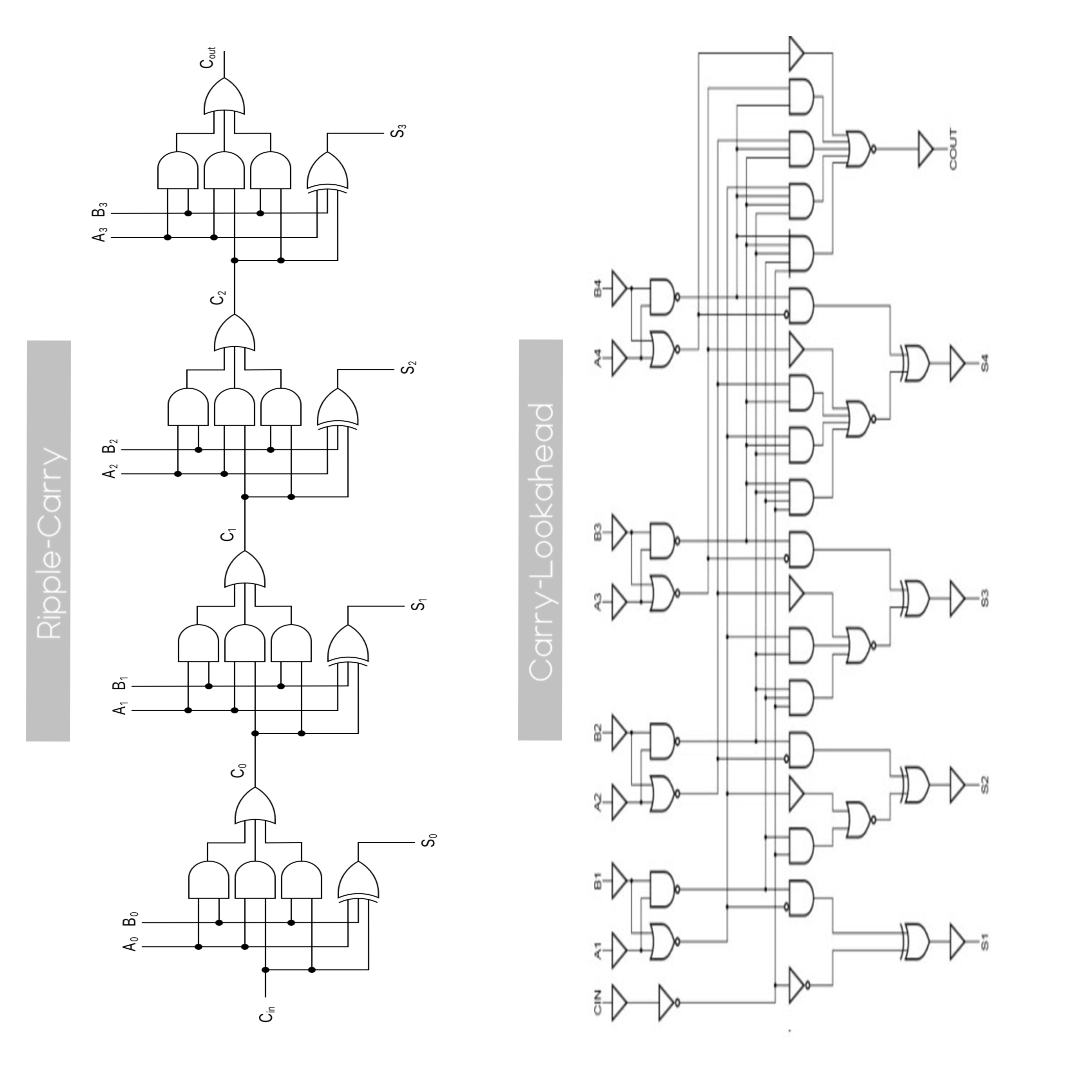
\includegraphics[width=0.5\textwidth, angle=270 ]{media/adders_comparison.jpg}
        \caption{Carry Lookahead Adder vs Ripple Carry Adder}
    \end{figure}
\end{frame}

\begin{frame}
    \frametitle{Let's do some math}
    \begin{equation}
 \resizebox{0.9\textwidth}{!}{%
            $
            \begin{aligned}
                &c_{in}[i+1]=c_{out}[i]=G[i] \ | \  (P[i] \ \& \ c_{in}[i])\\
                &c_{in}[i+1]=G[i] \ | \  (P[i] \ \& \ (G[i-1]  \ | \  (P[i-1] \ \& \ c_{in}[i-1])))\\
                &c_{in}[i+1]=G[i] \ | \  (P[i] \ \& \ (G[i-1]  \ | \  (P[i-1] \ \& \ (G[i-2]  \ | \  P[i-2] \ \& \ c_{in}[i-2]))))\\
                &c_{in}[i+1]=G[i] \ | \  (P[i] \ \& \ G[i-1])  \ | \  (P[i] \ \& \ P[i-1] \ \& \ (G[i-2]  \ | \  (P[i-2] \ \& \ c_{in}[i-2])))\\
                &c_{in}[i+1]=G[i] \ | \  (\sum_{j=1}^{i} (\prod_{k=j}^{i} P[k]) \  \& \ G[j-1]) \ | \  ((\prod_{k=0}^{i} P[k]) \ \& \ c_{in}[0])\\
                &\text{Notation: } i \geq j \text{ , } P[i, j] = \prod_{k=j}^{i} P[k] \\
                &c_{in}[i+1]=G[i] \ | \  (\sum_{j=1}^{i} P[i, j] \  \& \ G[j-1]) \ | \  (P[i, 0] \ \& \ c_{in}[0])\\
            \end{aligned}$%
 }
    \end{equation}
\end{frame}

\begin{frame}
    \frametitle{Carry Lookahead Adder Tree}
    \begin{figure}
        \centering
        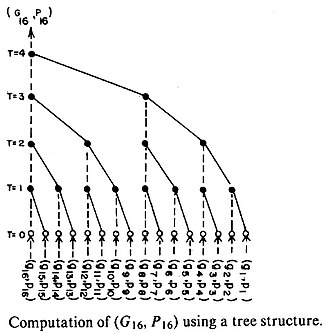
\includegraphics[width=0.5\textwidth]{media/cla_tree.jpg}
        \caption{Carry Lookahead Adder Tree}
    \end{figure}
\end{frame}

\begin{frame}
    \frametitle{Carry Lookahead Adder Kogge-Stone}
    \begin{figure}
        \centering
        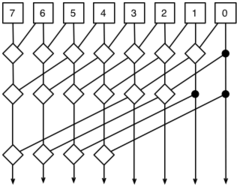
\includegraphics[width=0.6\textwidth]{media/Kogge-stone-8-bit.png}
        \caption{CLA Kogge-Stone}
    \end{figure}
\end{frame}

\begin{frame}
    \frametitle{Carry Lookahead Adder Brent-Kung}
    \begin{figure}
        \centering
        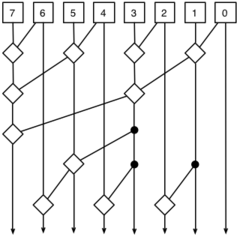
\includegraphics[width=0.6\textwidth]{media/Brent-kung-8-bit.png}
        \caption{CLA Brent-Kung}
    \end{figure}
\end{frame}

\begin{frame}
    \frametitle{Carry Skip Adder (bypass)}
    \begin{figure}
        \centering
        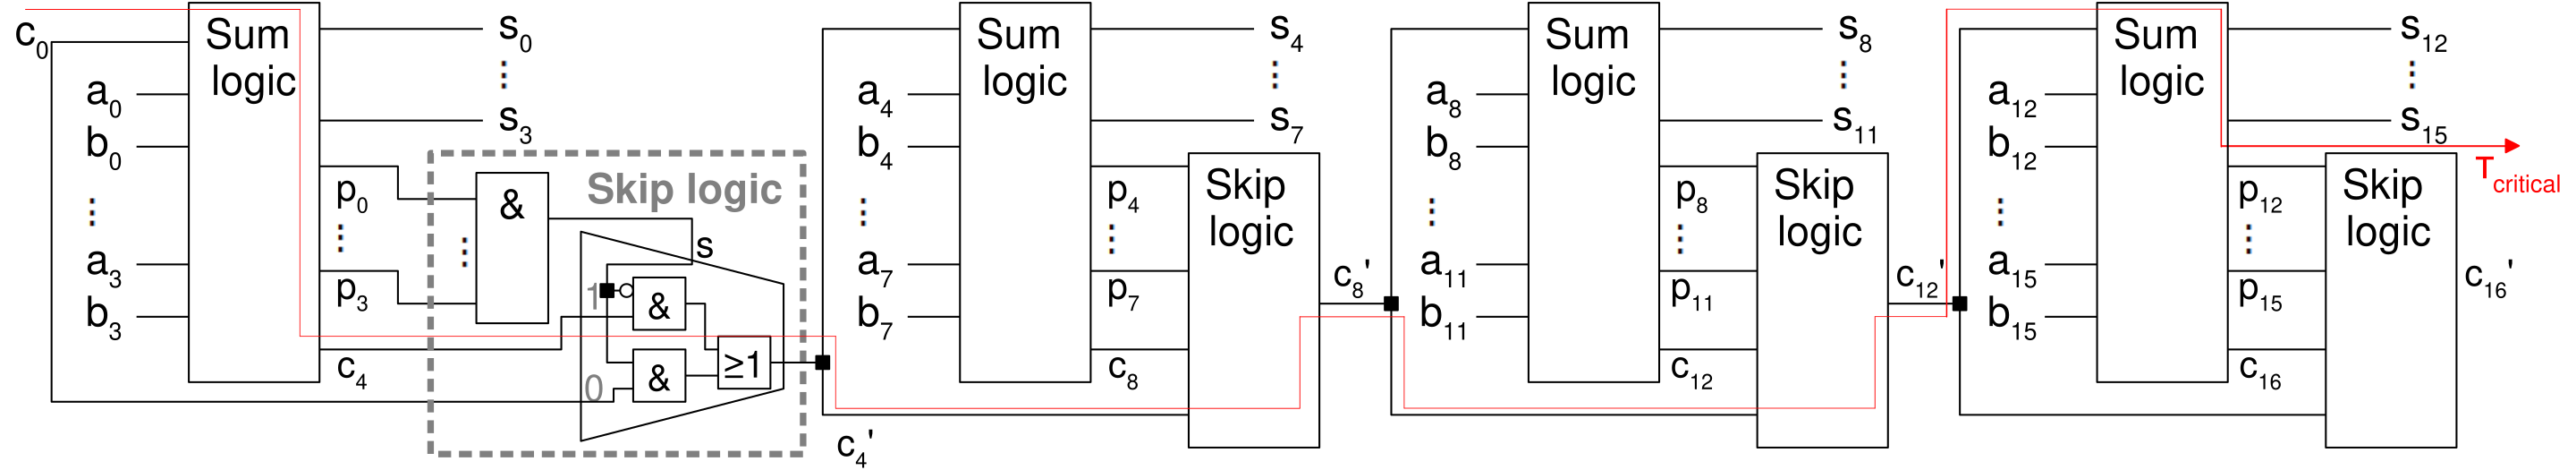
\includegraphics[width=0.9\textwidth]{media/BCSAdder16Bit.png}
        \caption{CSA 16-bit By Tibor89 - Own work, CC BY-SA 3.0, https://commons.wikimedia.org/w/index.php?curid=31748842}
    \end{figure}
\end{frame}

\begin{frame}
    \frametitle{Carry Select Adder (multiplexer)}
    \begin{figure}
        \centering
        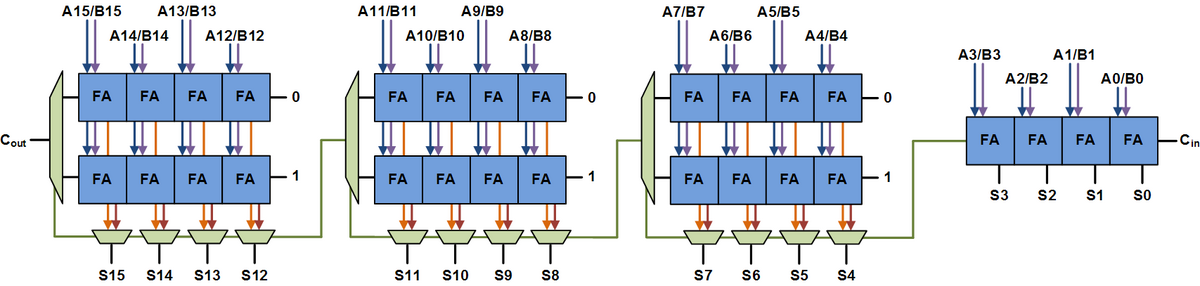
\includegraphics[width=0.9\textwidth]{media/Carry-select-adder-fixed-size.png}
        \caption{CSelectA 16-bit}
    \end{figure}
\end{frame}

% \begin{frame}
%     \frametitle{Exam Questions}
%  Template: Given the x-bit adder of type y, calculate the number of gates for the carry-out.

%  Example: Given the 8-bit ripple carry adder, calculate the number of gates for the carry-out.

%  Example: Given the 16-bit carry-lookahead adder Brent-Kung on 4-bits with Carry Skip adder, calculate the number of gates for the carry-out.
% \end{frame}

\subsection{MUL}

\begin{frame}
    \frametitle{Multiplication}
    \begin{equation}
        \begin{aligned}
            &P = M \times R\\
            &P=\sum_{i=0}^{n-1} (M \times R[i] \times 2^i)\\
            &P=\sum_{i=0}^{n-1} ((M \ \& \ \{n \times R[i]\}) \ll i)\\
        \end{aligned}
    \end{equation}
\end{frame}

\begin{frame}
    \frametitle{Let's do some math}
    \begin{equation}
        \begin{aligned}
            &P = M \times R\\
            &P = M \times 8'b0111_0011\\
            &P = M \times (2^6 + 2^5 + 2^4 + 2^1 + 2^0)\\
            &P = M \times (2^7 - 2^5 + 2^2 - 2^0)\\
        \end{aligned}
    \end{equation}
\end{frame}

\begin{frame}
    \frametitle{Booth's Algorithm}
 Booth's algorithm is a multiplication algorithm that multiplies two signed binary numbers in two's complement notation.
 The algorithm reduces the number of additions required for the multiplication of two numbers.
    \begin{equation}
        \begin{aligned}
            &|M|=|R|=n\\
            &|P|=2 \times n + 1\\
            &|M_{+}|=|M_{-}|=2 \times n+1\\
            &M_{+}=M \ll (n + 1)\\
            &M_{-}=-M \ll (n + 1)\\
            &-M=\overline{M}+1\\
            &|-M|=n\\
            &M_{+}=\{M, 0\}\\
            &M_{-}=\{-M, 0\}\\
            &P=\{0,R,1'b0\}\\
        \end{aligned}
    \end{equation}
\end{frame}

\begin{frame}
    \frametitle{Booth's Algorithm}
 Booth's Algorithm steps:
    \begin{equation}
        \begin{aligned}
            &P=\{0,R,1'b0\}\\
            &\text{for n steps}\\
            &\begin{cases}
 \text{if } P[1:0]=2'b01 \text{ then } P=P+M_{+}\\
 \text{if } P[1:0]=2'b10 \text{ then } P=P+M_{-}\\
 \text{otherwise } P=P\\
            \end{cases}\\
            &P=P \ggg 1\\
            &\text{end for}\\
            &result=P[(2 \times n):1]
        \end{aligned}
    \end{equation}
\end{frame}

% \begin{frame}
%     \frametitle{Exam Questions}
%  Template: Given the x-bit Booth's algorithm, how many additions are for $M \times R$?

%  Example: Given the 8-bit Booth's algorithm, how many additions are for $8'b0010_0110 \times 8'b1111_0110$?
% \end{frame}

\subsection{DIV/MOD}

\begin{frame}
    \frametitle{DIV/MOD Debate}In computer engineering, integer division is a debated issue.
    The next formulas define integer division:
    \begin{equation}
        \begin{aligned}
 \text{Dividend} &= \text{Divisor} \times \text{Quotient} + \text{Remainder}\\
 \text{Remainder} &= \text{Dividend} - \text{Divisor} \times \text{Quotient} 
        \end{aligned}
    \end{equation}
The following operations might help $(-5)/2$ and $5/(-2)$ might help to understand the debate.
 Taking the first one, $5=2 \times -3 + 1$, but another solution is $5=2 \times -2 + (-1)$.
 A similar choice is for the second one, $-5=-2 \times 3 + 1$ and $-5=-2 \times 2 + (-1)$.
\end{frame}

\begin{frame}
    \frametitle{DIV/MOD Debate}
We can categorize the following types of divisions \footnote{Modulo operation. (2022, November 16). In Wikipedia. https://en.wikipedia.org/wiki/Modulo\_operation}:
    \begin{itemize}
        \item Truncated division. $\text{Quotient}=[\frac{\text{Dividend}}{\text{Divisor}}]$ (round down). The remainder and the dividend have equal signs.
        \item Floored division. $\text{Quotient}=\lfloor \frac{\text{Dividend}}{\text{Divisor}} \rfloor$ (integer part). The remainder and the divisor have equal signs.
        \item Euclidean division.  The remainder is always positive. \par  $\text{Quotient}=\text{sign}(\text{Divisor}) \times \lfloor \frac{\text{Dividend}}{|\text{Divisor}|} \rfloor = \begin{cases}
             \lfloor \frac{\text{Dividend}}{\text{Divisor}} \rfloor & \text{if } \text{Divisor}>0\\
             \lceil \frac{\text{Dividend}}{\text{Divisor}} \rceil & \text{if } \text{Divisor}<0
        \end{cases}$
        \item Round division. $\text{Quotient}=\text{round}(\frac{\text{Dividend}}{\text{Divisor}})$
        \item Ceiling division. $\text{Quotient}=\lceil \frac{\text{Dividend}}{\text{Divisor}} \rceil$. The remainder and the divisor have opposite signs.
    \end{itemize}
\end{frame}

\begin{frame}
    \frametitle{Let's do some math for unsigned numbers}
    \begin{equation}
        \begin{aligned}
            &Q = \text{Dividend}\\
            &M = \text{Divisor}\\
            &R = \text{Remainder, Quotient}\\
            &|Q|=|M|=n\\
            &|R|=2 \times n\\
            &R=\{0,Q\}\\
            &|M_{+}|=|M_{-}|=2 \times n\\
            &M_{+}=M \ll n\\
            &M_{-}=-M \ll n\\
            &-M=\overline{M}+1\\
            &|-M|=n\\
            &M_{+}=\{M, 0\}\\
            &M_{-}=\{-M, 0\}\\
        \end{aligned}
    \end{equation}
\end{frame}

\begin{frame}
    \frametitle{Booth's Algorithm for non-restoring division for unsigned numbers}
    \begin{equation}
        \begin{aligned}
            &R=\{0,Q\}\\
            &\text{for n steps}\\
            &R=R \ll 1\\
            &\text{if } R[2 \times n - 1]=\begin{cases}
                1'b1 \text{ then } R=R+M_{+}\\
                1'b0 \text{ then } R=R+M_{-}\\
            \end{cases}\\
            &\text{if } R[2 \times n - 1]=\begin{cases}
                1'b1 \text{ then } R[0]=0\\
                1'b0 \text{ then } R[0]=1\\
            \end{cases}\\
            &\text{end for}\\
            &\text{if } R[2 \times n - 1]=1'b1 \text{ then } R=R+M_{+}\\
            &\text{Quotient}=R[n-1:0]\\
            &\text{Remainder}=R[2 \times n -1 : n]
        \end{aligned}
    \end{equation}
\end{frame}